\chapter{Course Introduction and What is Physics}
%\pagenumbering{arabic}

\section{Course Overview}
These lecture notes contain the same content as was covered during the lectures for \textbf{STM0005 Physics}, I will likely be updating them during the course so please check back regularly for the latest version. In particular, more figures will be added as these notes are updated. Many of the figures used in the lectures are hand drawn and it takes some time to produce good quality versions of them.\\


The lecture slides for week one contained information about the organisation of the module including a rough schedule for the module, an overview of how you will be assessed, and  how to contact me. I will not duplicate all of that here. If you have any questions during the module then you can send me an \href{mailto:rossc@edgehill.ac.uk}{email} or come by my office during the office hour times. The recommended and supplementary reading for the course are included in the reading list available on the module's virtual learning environment (VLE) page. I will occasionally cite one of the books in these notes if it is particularly relevant to look at it for that topic. The main reference for the course is \citep{breithaupt2016aqa} which covers the whole of the A-level physics curriculum.\\

This module does not cover the whole of A-level physics and we will mainly use the following chapters from \citep{breithaupt2016aqa}: 6, 7, 8, 9, 10, 12, 13, 17, and 18. For more background on some of the practical skills useful for the lab sessions chapters 14, 15, and 16 may be useful to look at as well.

\section{What is Physics}
\textbf{Physics} is the study of the natural world. It is the most basic of the sciences and underpins all of the others. It is typically pursued through constructing mathematical models of real world phenomena, using these to make predictions, then testing the predictions by carrying out experiments.\\

In this module we will spend time on both the theoretical and computational aspects of physics and carrying out experiments.  Hopefully you will find that the simple (and sometimes dull) problems that we will study in the lectures and tutorials are useful for building you intuition about real life phenomena. This is partly what the practical sessions are there for.\\

In the lab sessions you will carry out the experiments outlined in the lab manual. The goal is to collect data and then compare this against the theoretical description.\\

As physics is a rational discipline, it teaches you a way to approach problems and construct arguments that will be useful to you in your subject specific modules in semester two and during the rest of your degree.  In particular, you will learn how to unpack information from the statement of a problem and how to identify the relevant mathematical techniques needed to solve the problem.

\section{Measurements and Units}
We said above that one aim of physics is to describe the world by constructing predictive models, then test these models via experiment. To carry out experiments, and then match our computations to experiment, we need to understand how to describe these measurements. \\

Measurement is a process of computing the amount of an unknown quantity using a known quantity. For example when we want to measure the length of an object we use a ruler of a known length. How do we know the length of the ruler? Well, when the ruler was made it was made to a standard size and compared against a standard ruler. Where does the standard come from? Organisations like the \href{https://www.npl.co.uk/products-services/instruments/standard}{National Physical Laboratory} are involved in defining standards for measurements, including defining the meter. It used to be that the meter was defined in terms of the circumference of the Earth and there was a platinum bar kept in a vault in Paris. This was the international standard for a meter with every other country taking their standard meter over to compare the length and check that what they called a meter was really a meter long. Now a meter is defined in terms of the speed of light and the distance that light travels in a second. This is much easier to check against as you no longer have to travel, though the visits to Paris must have been nice.\\

If you want to know more about the history of measurement and where the units that we use come from then I recommend reading \citep{vincent2022beyond}.

There are standards like this for all of the physical quantities that we want to measure: length, mass, charge, and all the others. \\


This reference standard tells us the physical units that we will use, for length this is the meter or m, we then get another part of the measurement which is the number of things with the size of the standard unit that we need to make the object we are measuring. For example. if we measure a table to be 2m long it means that we need two standard meters next to each other to get something as long as the table. The two parts of the measurement are also called:
\begin{itemize}
\setlength{\itemsep}{-5pt}
    \item the magnitude or numerical value, in this case 2,
    \item and the reference standard or unit of measurement, in this case the meter.
\end{itemize}

It is important to know that in physics, if you quote a measured value and do not include the units of measurement then the measurement is \textbf{meaningless}. This is because anyone that you tell this measurement to will not know what the appropriate units are. For example if you quoted the length of a table to be 2. How do we know whether this means 2 m, 2 cm, 2 yd, or if you have created your own unit of measurement\footnote{This may sound ridiculous but an MIT student called Oliver Smoot did just this when measuring the length of a bridge in Boston. See \href{https://en.wikipedia.org/wiki/Smoot}{here} for the story.}. In this module you need to always include the correct units when providing numerical answers to questions.\\

Importantly there are different types of units. Units like the meter for length, the second for time, the kilogram for mass, etc, are called \textbf{fundamental units} as they are defined independently of other quantities.  There are also \textbf{derived units}, like the Joule for energy, the Newton for force, and many others. Derived units are expressed in terms of fundamental units, for example a force is a mass times an acceleration (See Newton's second law in Week 4) so the Newton is equal to kilograms meters per second squared. In symbols this is expressed as $\text{N}=\frac{\text{Kg m}}{\text{s}^{2}}$.\\

There are also \textbf{supplementary units} which are measurements of angles like radians (rad) and steradians (Sr.).\\

The system of units used in this module, and almost everywhere, is known as the \textbf{International System of Units} or SI. It has base units including seconds, meters, and kilograms. There are other systems of units such as cgs, where cm, grams, and seconds are used as the base units.\\

When measuring length we are also familiar with using different units depending on the scale of the quantity. For example small objects may be measured in cm while large objects would be measured in m or km. The prefix has an important roll as it tells us the power of ten that is in front of the unit. Everyone is likely to know that there are 100 centimetres in 1 metre and 1000 metres in a kilometre. In terms of symbols we would write this as:
\begin{align*}
    100 \text{cm} &=1 \text{ m},\\
    1000 \text{m} &= 1\times 10^{3} \text{m} = 1 \text{km},\\
    1 \text{cm} &= 0.01 \text{m} = 1\times 10^{-2} \text{m}.
\end{align*}

This is what the k in kilograms stands for, 1 kg = 1000 g. There are many more prefixes for orders of magnitude, they are summarised in Table \cref{table:1}.

\begin{table}[ht]
\centering
\caption{The powers of ten along with their names and the symbol used as a prefix. The usual rule of thumb is positive powers of ten have capital letter prefixes while negative powers of ten have lower case prefixes. the use of k for kilo is the only exception to this pattern.}

\vspace{4mm}

\label{table:1}



\begin{tabular}{|c|c|c|} 
 \hline
 \textbf{Power of Ten} & \textbf{Name} & \textbf{Symbol}\\
 \hline
 $10^{15}$ & Peta & P \\
 \hline
$10^{12}$ &	Tera & T \\
\hline
$10^{9}$ &	Giga & G	\\
\hline
$10^{6}$ &	Mega & M	\\
\hline
$10^{3}$ &	Kilo & k	\\
\hline
$10^{-2}$ &	centi & c	\\
\hline
$10^{-3}$ &	milli & m \\
\hline
$10^{-6}$ &	micro & $\mu$	\\
\hline
$10^{-9}$ &	Nano & $\eta$ or n	\\
\hline
$10^{-12}$ &pico & p\\
\hline
\end{tabular}
\end{table}

Recall that sometimes $10^{\text{number}}$ is called \textbf{Scientific notation}. The superscript is called the \textbf{index} or \textbf{exponent}. It is important to remember how to work with indices mathematically (see the first tutorial sheet for questions about this). The most important rules to remember are that:

\begin{equation*}
    a^{0}=1, \qquad a^{-b}=\frac{1}{a^{b}}.
\end{equation*}
These say that any number raised to the power of zero is one, and a number raised to a negative power is the same as one over the same number raised to the positive power.

\section{Fermi Problems and Approximations}


\begin{figure}[ht]
\centering
    %\pdftooltip{
    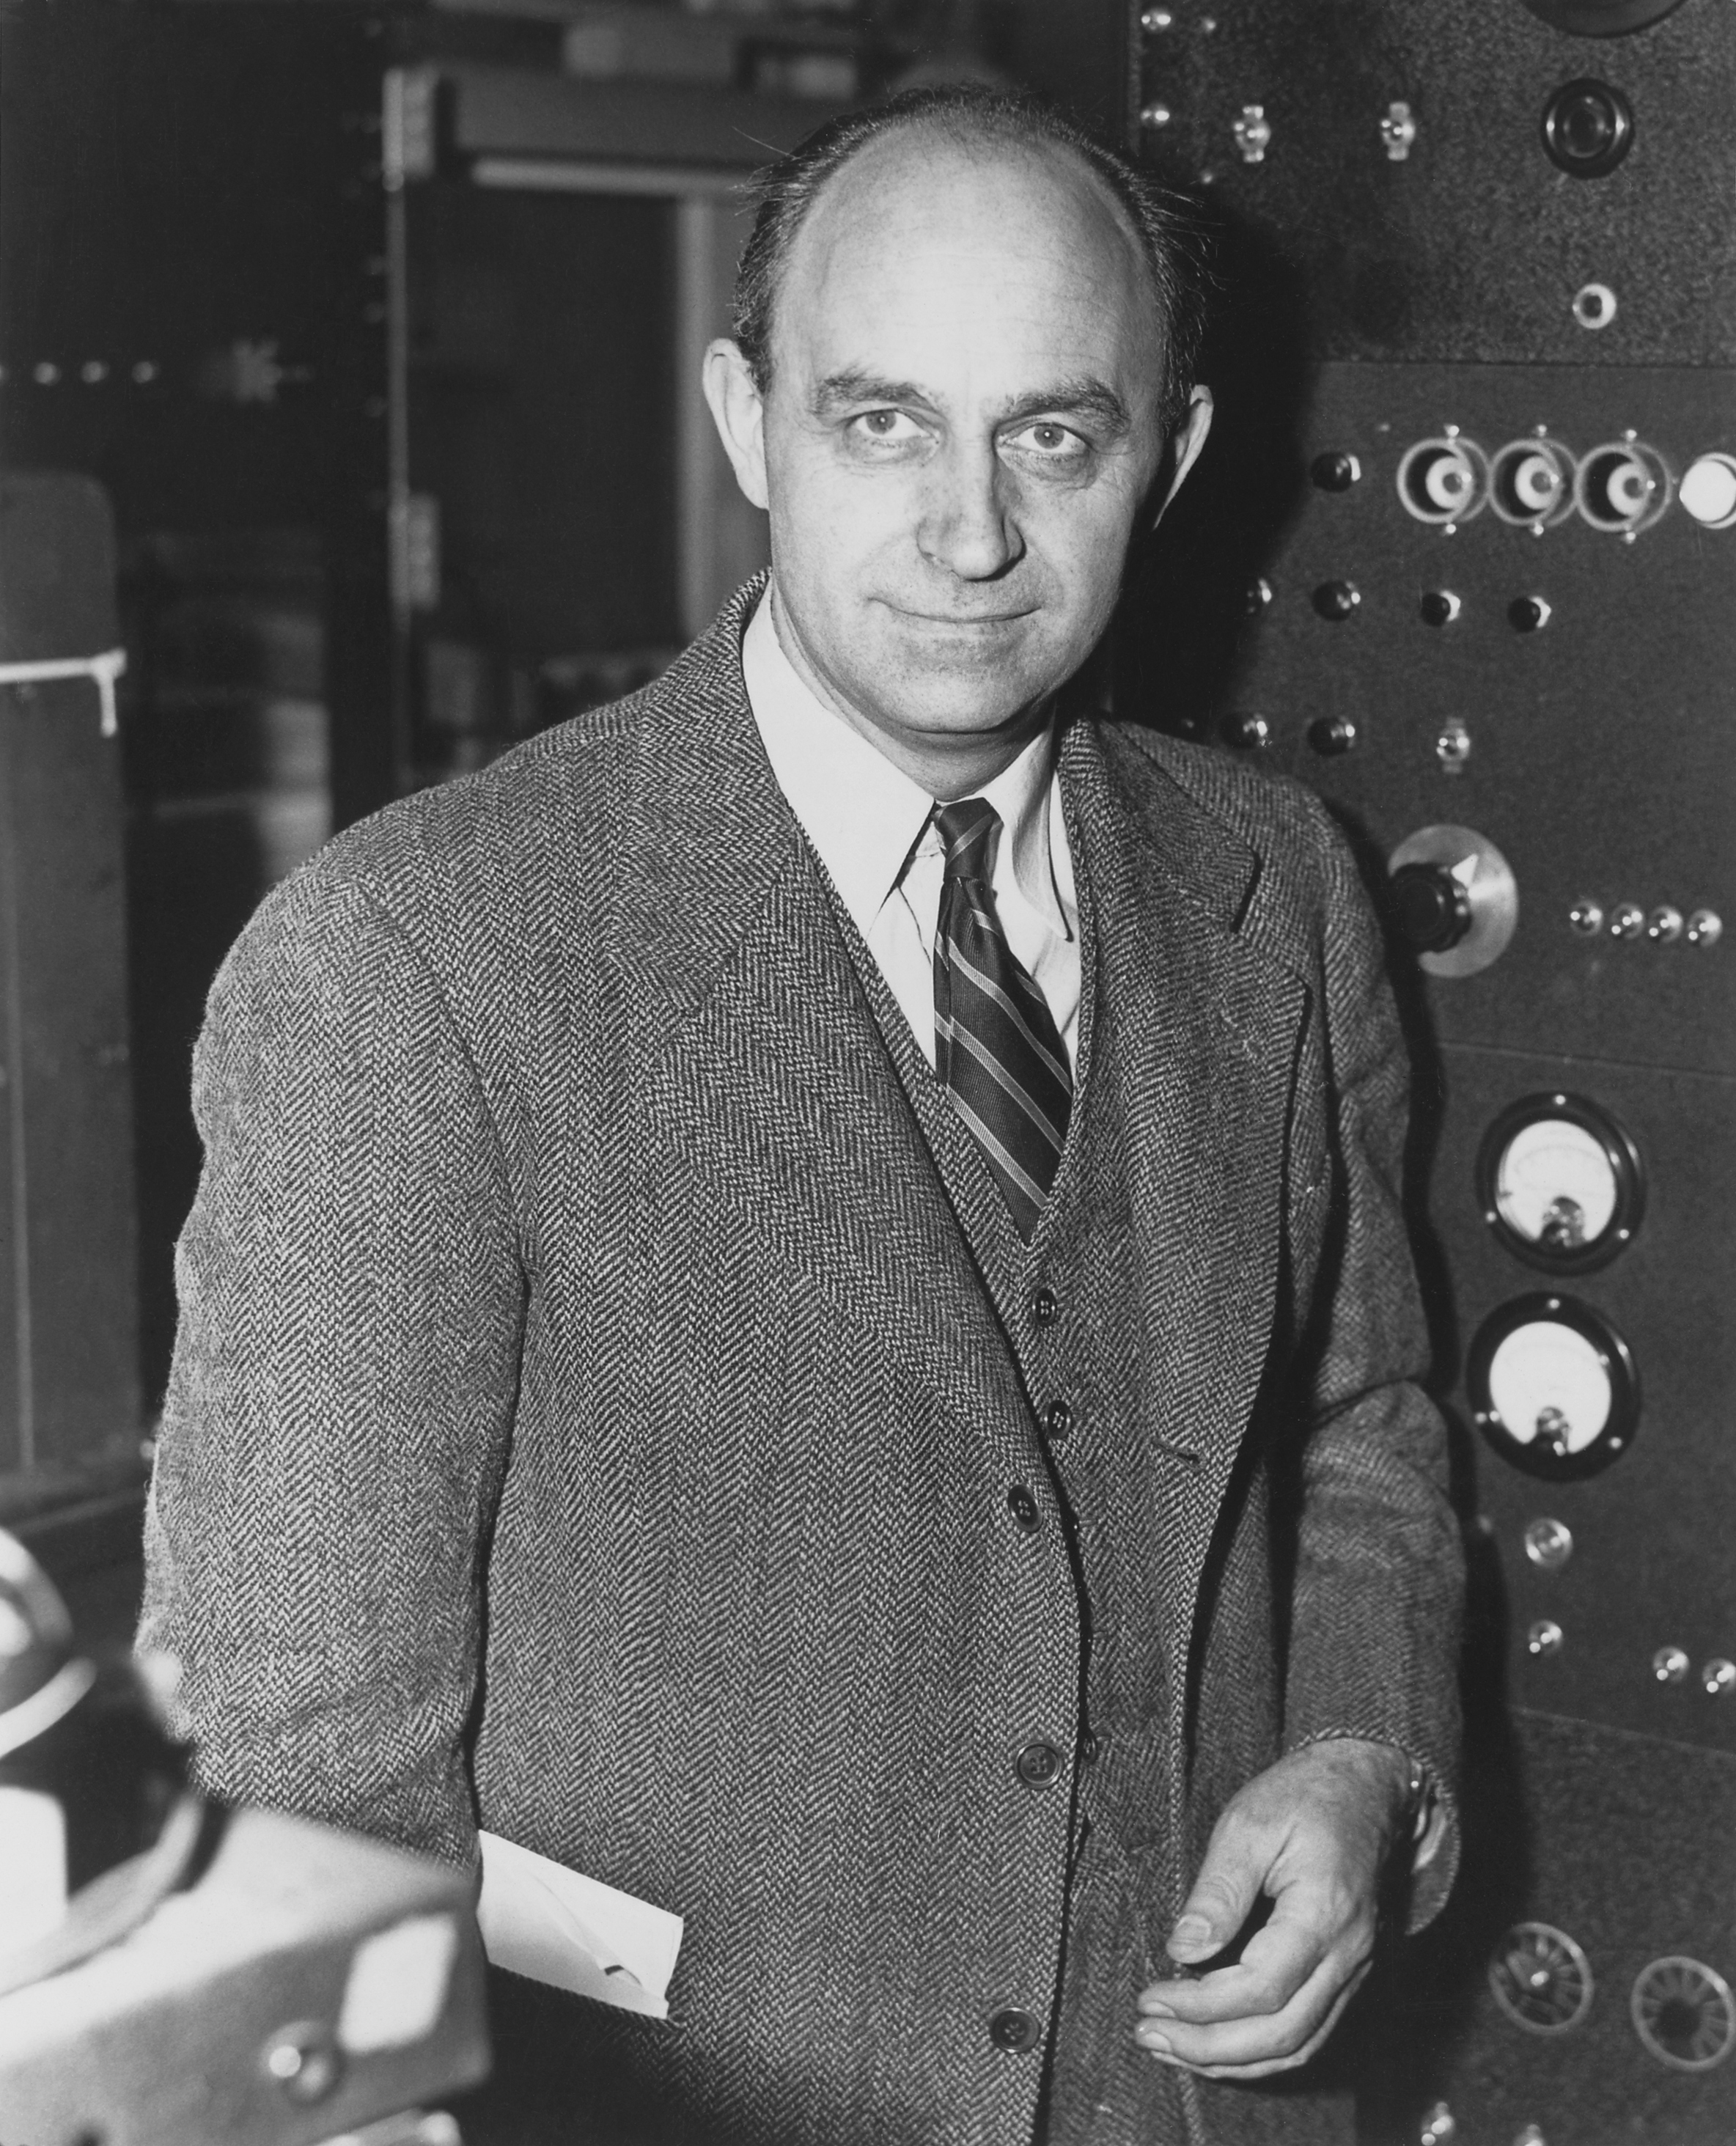
\includegraphics[width=0.4\textwidth, alt={A picture of the Italian-American physicist Enrico Fermi from Wikimedia commons.}]{figures/Enrico_Fermi_1943-49.jpg}
    %}{A picture of the Italian-American physicist Enrico Fermi from Wikimedia commons.}
    \caption{The Italian-American physicist Enrico Fermi from \href{https://commons.wikimedia.org/wiki/File:Enrico_Fermi_1943-49.jpg}{Wikimedia Commons}.}
\end{figure}

While much of physics is about making very precise measurements such as the high energy physics experiments being conducted at CERN, or the measurements of the fundamental constants used to define measurement standards. A lot can be understood by working roughly and making approximations. \\

The standard example of this style of estimation is asking how many piano tuners there are in a certain city. In the lectures we treated the case of London and Ormskirk. This style of approximation problem is often called a \textbf{Fermi Problem} after the physicist Enrico Fermi who liked to ask questions like ``How many piano tuners are there in Chicago?'' Famously Fermi estimated the yield of the first atomic bomb by dropping a scrap of paper and seeing how far it was blown and making some estimates. 

\paragraph{Example 1.1} How many piano tuners are there in London? To answer this start by making a few estimations:
\begin{itemize}
\setlength{\itemsep}{-5pt}
    \item the population of London, around 9 Million people,
    \item how many people have a piano, around 1 in 50,
    \item how often does a piano need tuned, around once a year,
    \item how many pianos can a piano tuner tune in a year, assume 5 a day 230 days a year\footnote{This is potentially the roughest estimate as I know piano tuners who only tune one piano a day, but that is not in a city.}. 
\end{itemize}

Putting this together we then calculate the number of piano tuners as
\begin{align*}
    \text{Number of Piano Tuners} &= \frac{\text{Population of London }}{\text{Number of people per piano} \times \text{Number of tunings a year}}\\
    &=\frac{9\times 10^{6}}{50\times 5\times 230}\simeq 160
\end{align*}

\paragraph{Question 1:}Can you estimate how many piano tuners there are in Ormskirk? Think about how the numbers would change in the above example.\\




\section{The Scientific Method}

In the earlier sections we have alluded to how physics works, constructing a model and then testing it against experiment. This is a very rough description of the \textbf{Scientific Method} which you will meet again in your subject specific modules in semester two and later in your degree. A schematic representation of the scientific method is given in \cref{fig2: scientific method}.


\begin{figure}[ht]
\centering
    %\pdftooltip{
    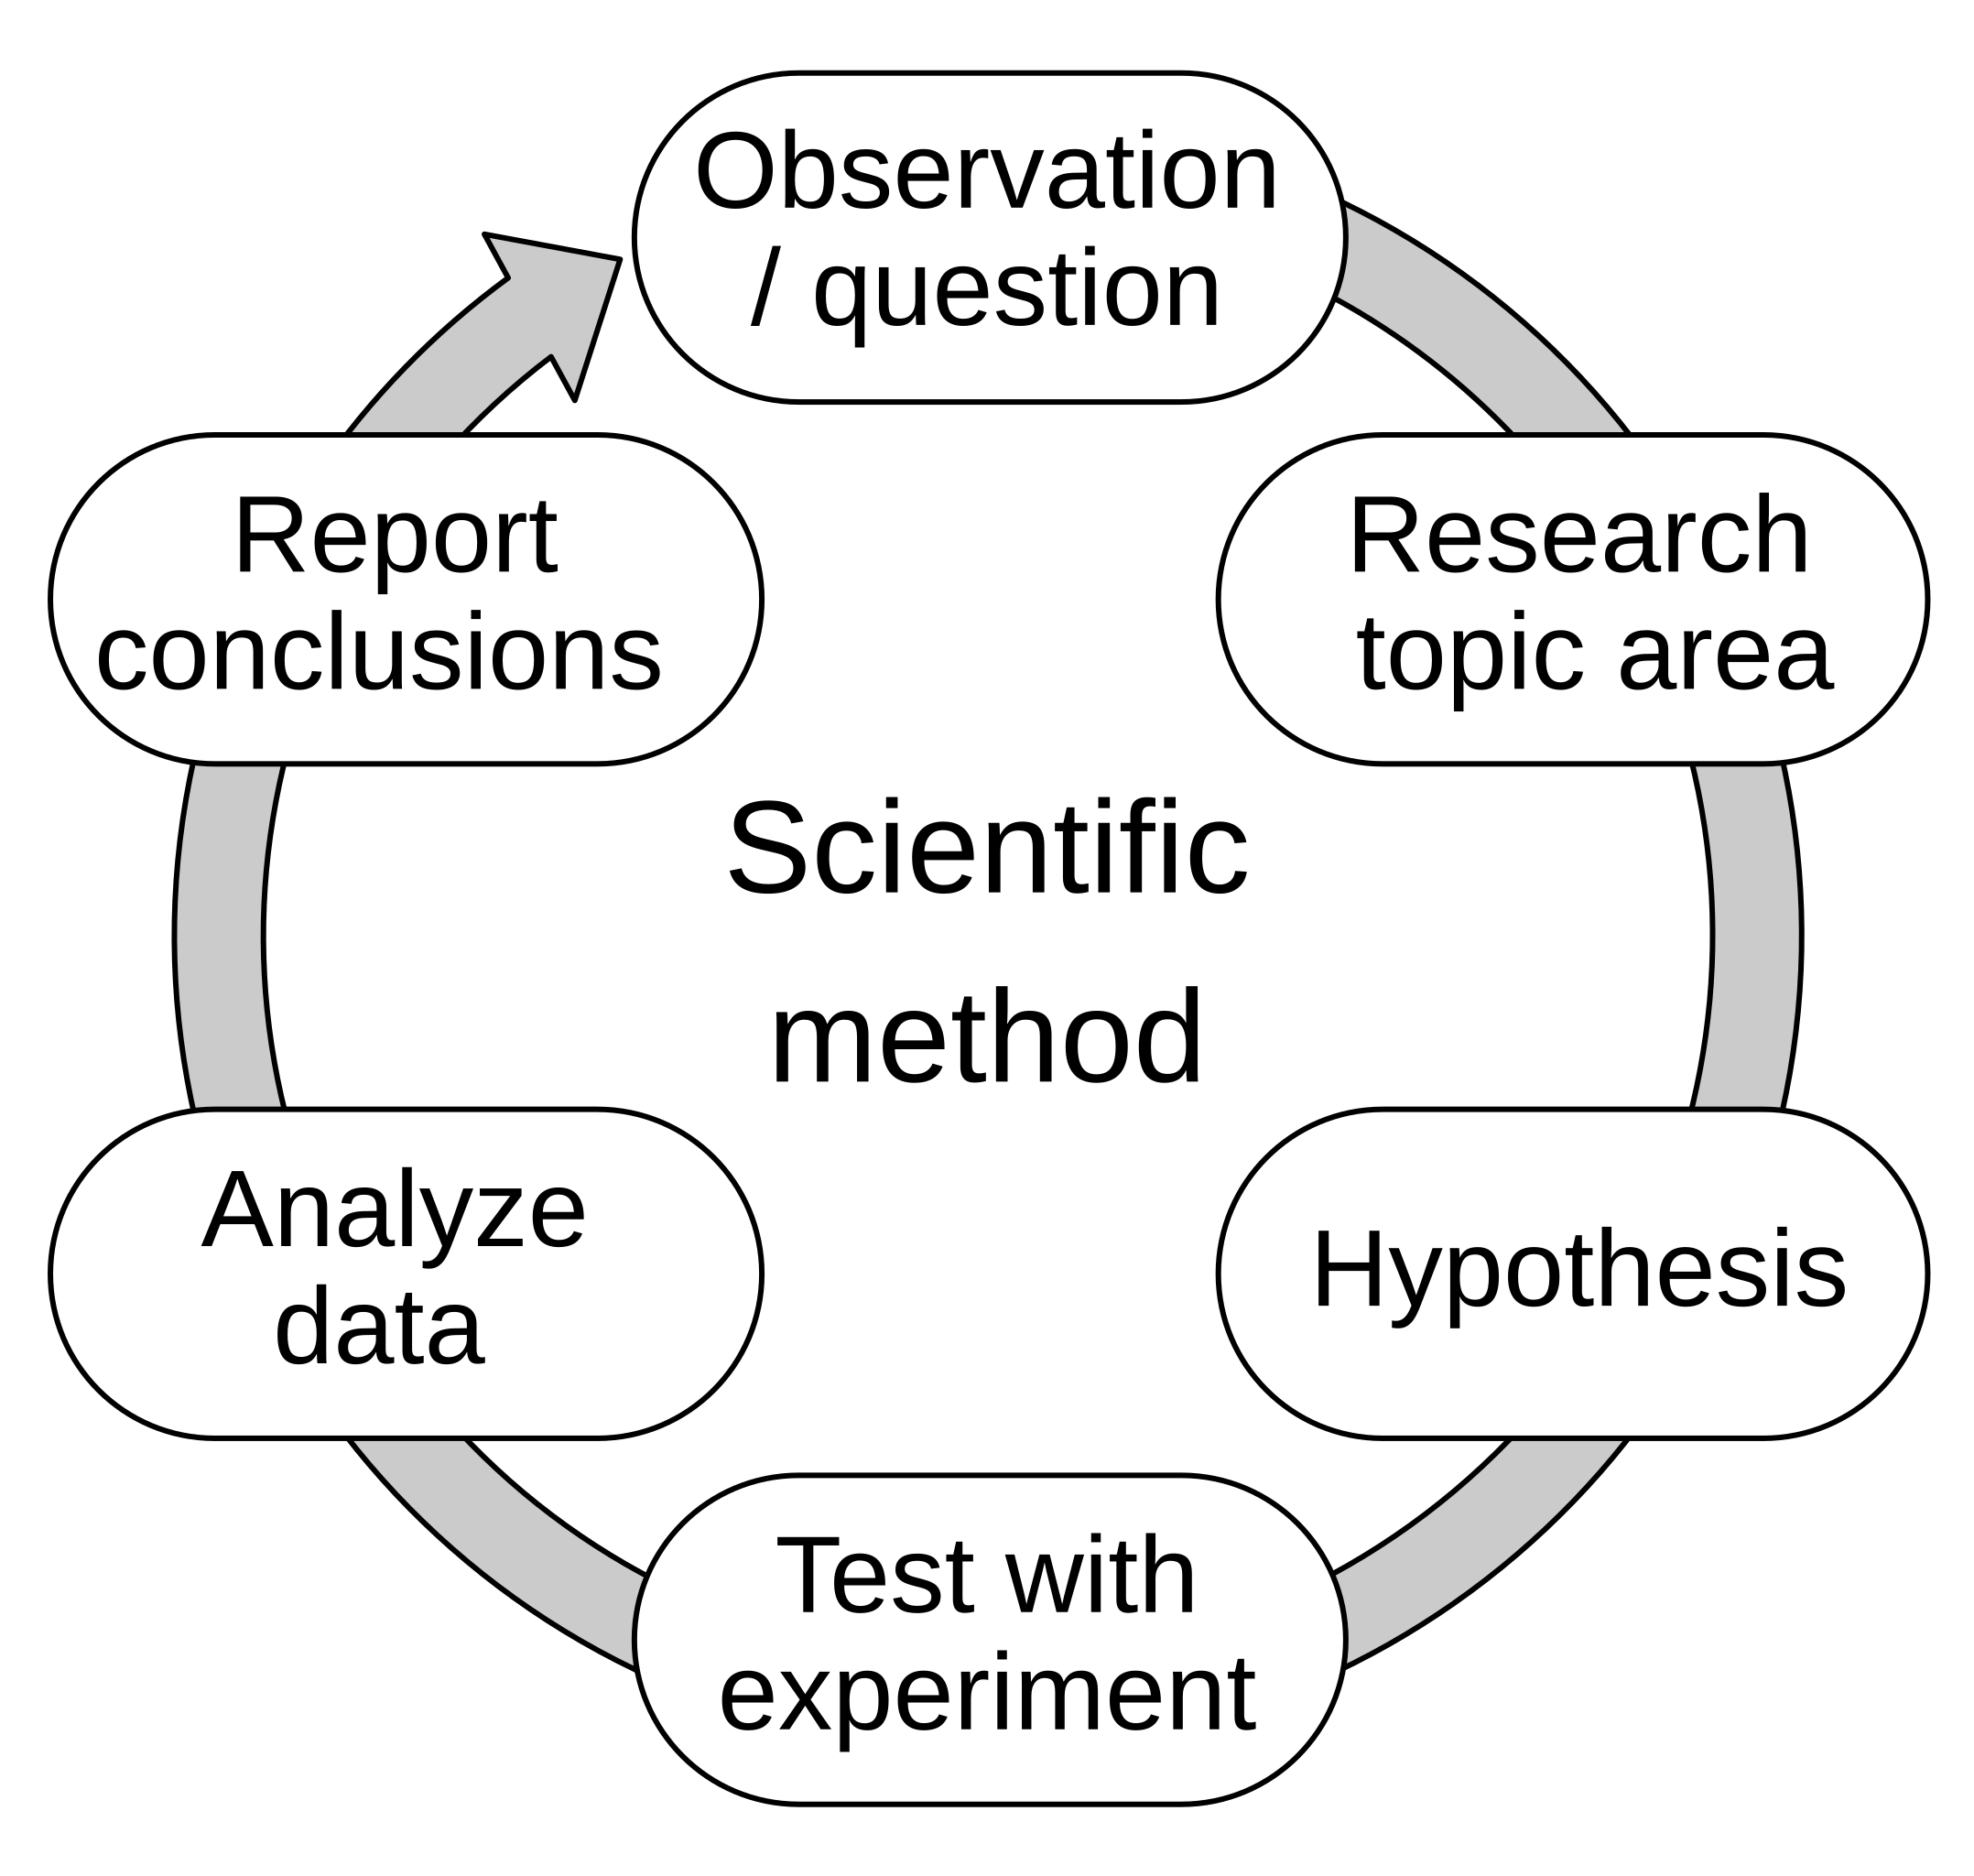
\includegraphics[width=0.6\textwidth,alt={A schematic of the scientific method as a cycle, image from Wikimedia commons.}]{figures/The_Scientific_Method.png}
    %}{A picture showing the scientific method from Wikimedia commons CC BY-SA 4.0 Efbrazil.}
    \caption{A representation of the scientific method from \href{https://commons.wikimedia.org/wiki/File:The_Scientific_Method.svg}{Wikimedia Commons} CC BY-SA 4.0 Efbrazil.}
    \label{fig2: scientific method}
\end{figure}

The process of the scientific method involves three main stages:
\begin{itemize}
\setlength{\itemsep}{-5pt}
    \item Making conjectures (hypothetical explanations) -- these may be mathematical models or just a description of your expectations.
    \item Deriving predictions from the hypotheses as logical consequences -- e.g. think about what your model/ expectations imply will happen.
    \item Carry out experiments or empirical observations based on those predictions -- this means test that reality matches your predictions.
\end{itemize}

This is an empirical method for acquiring knowledge and involves careful observation while applying rigorous scepticism about what is observed. The reason for the scepticism is that you are essentially watching something happen, making a guess why it happens, then testing your guess. It is easy to be biased and think that you have confirmed your guess even if the experiment does not show this. One then formulates a hypothesis, or hypotheses, based on the observations, before refining or eliminating hypotheses based on the experimental findings.\\

Hypotheses enable predictions to be made about outcomes based on observations. A good hypothesis is not just a guess since it can be rigorously tested against an experiment or observation. Hypotheses can be strengthened by using different research methods to carry out and analyse your experiment, e.g. surveys, experiments, statistical analysis, literature review, etc.\\

An effective hypothesis is usually one concise sentence containing the following specific elements:

\begin{itemize}
\setlength{\itemsep}{-5pt}
    \item A prediction:
    \begin{itemize}
\setlength{\itemsep}{-5pt}
    \item An `if/then' statement
    \item A declarative statement
    \item The statement must be what the research is setting out to test
\end{itemize}
    \item Variables:
    \begin{itemize}
\setlength{\itemsep}{-5pt}
    \item Clearly state all the variables that will be considered in the study
    \item Designing an experiment using these variables can prove or disprove the prediction
\end{itemize}
    \item Subject group: 
    \begin{itemize}
\setlength{\itemsep}{-5pt}
    \item State the subjects to be tested during the research
\end{itemize}
\end{itemize}

\paragraph{Example 1.2:}Imagine you are walking in the country side and go past a field with some sheep. If all the sheep that you see are white you may come up with the hypothesis that ``All sheep have white wool''. In this case the subjects are the sheep, the variables are the colour of the wool, and the prediction is that all sheep have white wool. If you keep walking and pass another field where the sheep have multiple colours of wool, say white, brown, and black, then you observe that your hypothesis is false.

\paragraph{Question 2:} How could you refine your hypothesis using the new data that you have taken? Can you tests this refined hypothesis in the same way?\\

During the practical sessions in this module you will carry out experiments, using the scientific method and following the details in the lab manual, and then write up your findings. An important part of scientific writing is putting your work in context and explaining how it connects to the existing literature. To be able to do this you need to build awareness of the existing scientific literature. This may be by looking at the module reading list, reading these lecture notes, looking up the topic online, or any other way to explore what is already known.\\

Remember, science is a continually evolving field; new discoveries and experiments are based on earlier work carried out by other scientists. Any literature that is read and used for inspiration should be referenced by stating how the previous work is related to what you have done. For this module the referencing should be done using the Edge Hill Harvard referencing style, there is information about this on the module's VLE page. \\

When writing up your work you need to be aware that scientific writing is not the same as writing an essay. The key features of scientific writing are: precision, clarity, formal language, and organisation. 

\paragraph{Precision:} Scientific writing relies on unequivocal accuracy, anyone reading it needs to be able to trust what you have written. This means that you need:
\begin{itemize}
\setlength{\itemsep}{-5pt}
    \item \textbf{Objectivity:} take an objective viewpoint towards the subject, the author does not just state their opinion. Relevant facts should be presented, justified, and analysed.
    \item \textbf{Thoroughness:} include as many details as are necessary for readers to thoroughly understand the subject. This is a delicate balance as you should not write too much or it can confuse the reader.
    \item \textbf{Exact language:} the use of figurative or imaginative language should be minimised; words and phrases should be used to convey their literal meaning.
\end{itemize}

\paragraph{Clarity:}A clear and consistent writing style is also important for establishing a trusted voice within the scientific community. It enables others to read your work and replicate any experiments that you have carried out.
\begin{itemize}
\setlength{\itemsep}{-5pt}
    \item The writer should clarify the meaning of any uncommon terms.
    \item The goal of the writing is to clearly explain the work that has been carried out so the results or observations should be summarised in a way that anyone can understand.
    \item The experiment and its results are fully explained.
    \item A consistent system of units are used and this choice is clearly explained. In this module and almost everywhere this choice of units is the SI system.
\end{itemize}

\paragraph{Formal language:}
\begin{itemize}
\setlength{\itemsep}{-5pt}
    \item This maintains professionalism.
    \item Slang and idioms should not be used. Some people also dislike the use of contractions.
    \item Make sure to use proper punctuation and grammar.
    \item The use of common language can help your work appeal to a larger audience. Think about the words and phrases that are used and make sure that they are appropriate, e.g. have you used any synonyms for simple words that could be used instead.
    \item Stick to either British or American English, do not mix words and spellings from the two.
\end{itemize}

\paragraph{Organisation:} Most scientific retaining follows a clear organisational structure. What that structure is depends on the discipline. During this module we will use the following structure:

\begin{itemize}
\setlength{\itemsep}{-5pt}
    \item \textbf{Introduction:}
    \begin{itemize}
\setlength{\itemsep}{-5pt}
    \item Relevant background information required to understand the purpose and findings of the work should be summarised.
    \item The purpose and unique value of the experiment or observation should be explained.
\end{itemize}
    \item \textbf{Materials and methods:}
    \begin{itemize}
\setlength{\itemsep}{-5pt}
    \item Explain how the study or experiment was conducted. e.g. what equipment was used, how did you set it up, describe how you made the measurements.
    \item There needs to be enough detail that someone else could replicate your experiment based on the description.
\end{itemize}
    \item \textbf{Results:}
    \begin{itemize}
\setlength{\itemsep}{-5pt}
    \item Give an objective explanation of the experimental results.
    \item Summarise the relevant quantitative and qualitative data. e.g. use appropriate charts and graphs to display your results.
\end{itemize}
    \item \textbf{Discussion:}
    \begin{itemize}
\setlength{\itemsep}{-5pt}
    \item Give an interpretation of the potential implications of your findings. e.g. how does it compare to your hypothesis or to existing theory. 
    \item Evaluate your results and discuss all of the possible interpretations.
    \item Give an outline for any potential future studies and say what you would do differently, and why, if you were to conduct the experiment again.
    \item Consider potential sources of inaccuracy in your results and talk about why these are present and how they could be minimised.
\end{itemize}
    \item \textbf{Conclusions:} The main points of the report are reiterated and the work is summed up.
\end{itemize}

As part of the assessment for the module you need to write up two of the experiments that you have carried out. The description of the coursework contains an outline of how to structure your work using the organisational style given above.